\documentclass{article}
\usepackage[utf8]{inputenc}
\usepackage{graphicx}


\begin{document}

\maketitle

\section{Team work}

In the development process, we take agile development. Our team is divided into two groups, Qilin Zhou is responsible for the Android side and Letao Wang and Lili Chen are responsible for the desktop side. All team members will have a one-hour meeting on Thursday 1pm to communicate the progress of each group and the plan for the next week. The main location is on the sixth floor of the bush house SE. Everyone at the meeting will talk about what they have done in the last week. Also have a brief introduction of the progress of the Android side and desktop side so far. In addition, we also explore the difficulties encountered in our development process and members of the group are go to help others to solve these difficulties. At the last 3 weeks, Siva is responsible for server configuration.\newline

The weekly meeting for Android is scheduled for Friday afternoon, and the desktop meeting is scheduled on Wednesday afternoon. The person who responsible for this part are worked together to develop the project and solve the problem together. The location of both side’s meeting is usually on the sixth floor of the bush house.\newline

In normal times, we communicate through the WhatsApp communication software, and notify the meeting time and place on WhatsApp. Sometimes, you can also seek help from other members of the team through WhatsApp, so that you can solve the problem remotely and in time.\newline

During the development process, all the code and files of the projects are shared by git command. When a team member uploads a new file, it needs to send a request to the other members of the team. The file can be merged into master after two team members are approved this. Sometimes the team members will make some suggestions for the uploaded documents, and the person who uploads the files will make changes according to the recommendations. If they do not modify, they will give reasons. The file can be merged into the master after two group members approved.\newline

The five images below reflect the contribution of each member in the team during project development process. Basically, our team have four team members (Letao Wang, Lili Chen, Siva, Qilin Zhou) focus on the project development.\newline


\begin{minipage}
\centering
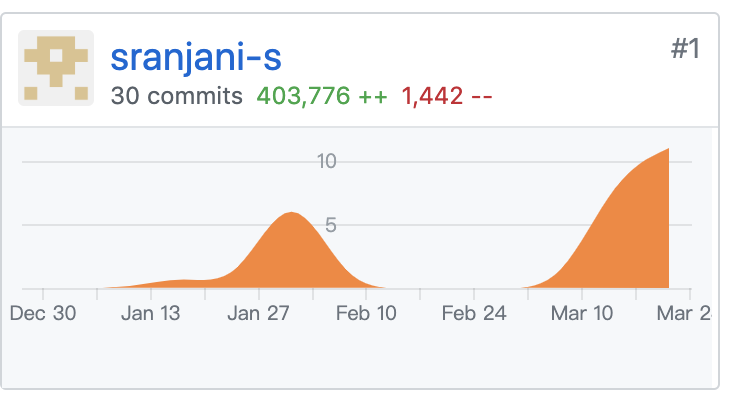
\includegraphics[scale=0.5]{siva.png}
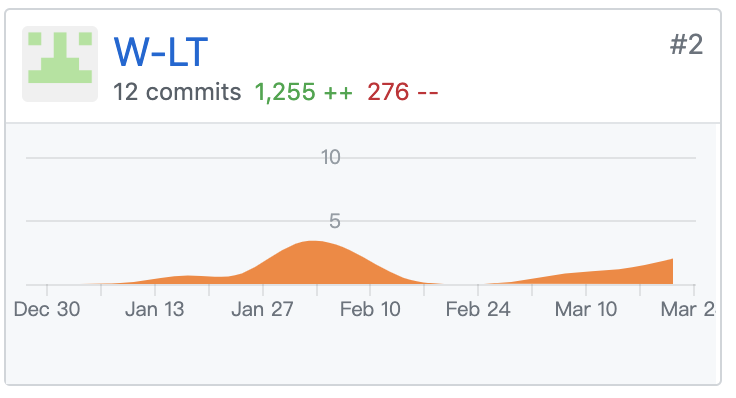
\includegraphics[scale=0.5]{Letao.png}
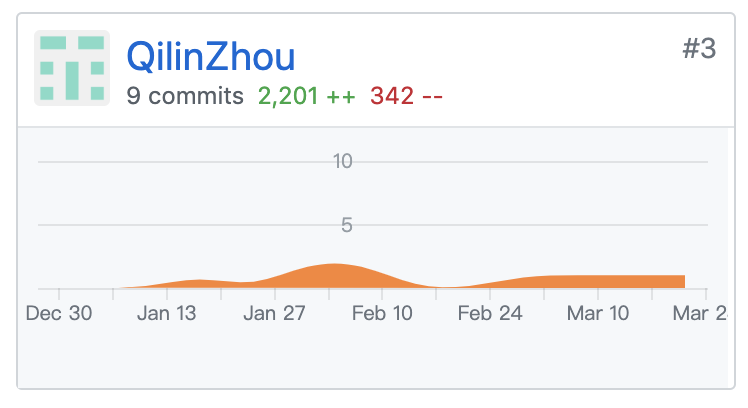
\includegraphics[scale=0.5]{Qilin.png}
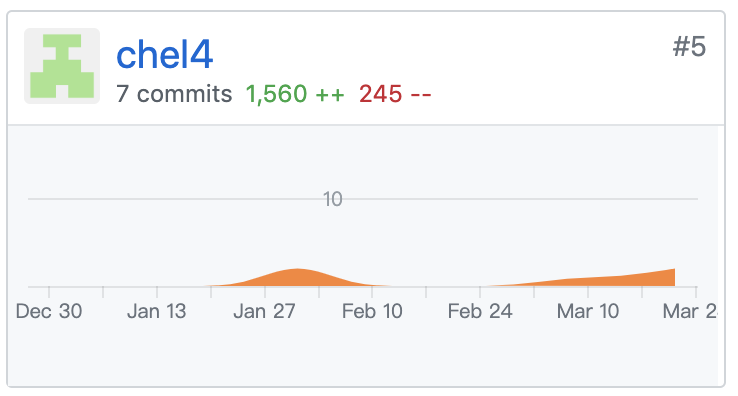
\includegraphics[scale=0.5]{Lili.png}
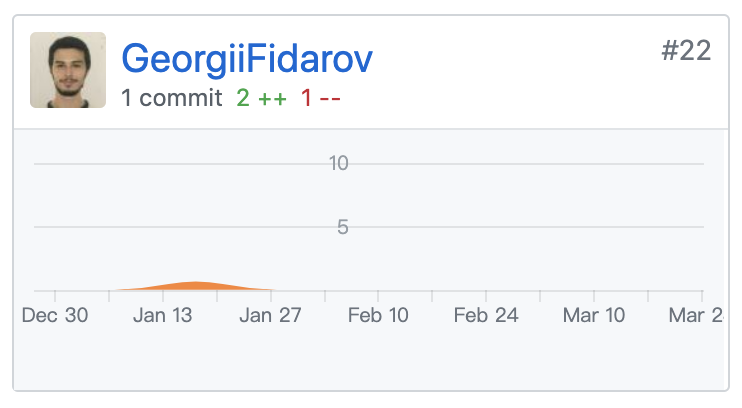
\includegraphics[scale=0.5]{georgii.png}
\label{fig:contribution in each team members}
\end{minipage}

The picture below shows the pulse in the GitHub from 27 February 2019 to 27 March 2019 in our team. From the data in the pulse, we can know that excluding merges, 4 authors have pushed 33 commits to master and 33 commits to all branches. What’s more, on master, 3,294 files have changed and there have been 406,303 additions and 0 deletions.\newline

\begin{minipage}
\centering
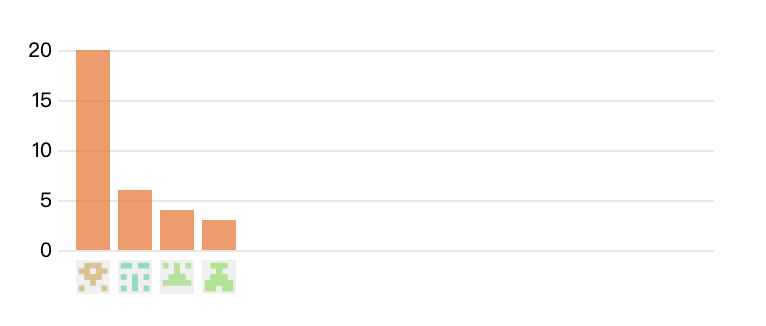
\includegraphics[scale=0.5]{pulse.png}
\label{fig:number of pulse}
\end{minipage}


The picture below shows the number of commits our team have made in a week. In the most case, we continued to make commits. Only in the period in the end of February, the commits is less. During project development, our team has a maximum of 20 commits in a week.\newline

\begin{minipage}
\centering
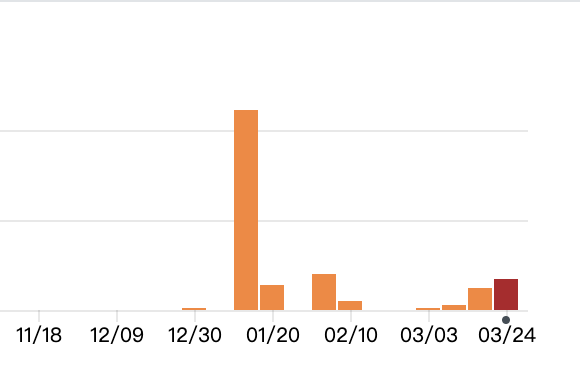
\includegraphics[scale=0.5]{commits.png}
\label{fig:Number of commits}
\end{minipage}

\end{document}
